\documentclass[a4paper,12pt]{scrartcl}
\usepackage[ngerman]{babel}
\usepackage[utf8]{inputenc}
\usepackage[verbose]{placeins}
\usepackage{lmodern}
\usepackage{amssymb}
\usepackage{graphicx}
\usepackage{amsmath}
\usepackage{multicol}
\usepackage{enumerate}
\usepackage{verbatim}

\usepackage{float}
%\usepackage{epstopdf}
\usepackage{longtable}
\usepackage{epsfig}
 \usepackage{placeins}
\usepackage{scrpage2}\pagestyle{scrheadings}
\title{Visualisierung der Abläufe des Parallelisierten PDE-Solvers}
\author{Johannes Timm \and Guannan Hu}
\date{\today}
% \chead{\titleinfo}
% \ohead{\today}
% \setheadsepline{1pt}
% \setcounter{secnumdepth}{0}
% \newcommand{\qed}{\quad \square}

\begin{document}
\maketitle
\notag

\section{Visualisierung der Implementierung des Gauss-Seidel und Jacobi Iterationsverfahrens}
\subsection{Konfiguration}
Für alle Tests wurden 20 Iterationen und ein Abbruch nach Iterationen gewählt. Damit einzelne Iterationsschritte erkennbar werden wurden 1000 Interlines gewählt. Um die Konfiuration der Knoten  odrungsgemäß abzuwickeln wurden die Jobscripte aus de vorherigen Aufgabe angepasst.
\subsection{Jacobi}
\subsubsection{2 Knoten 3 Prozesse}

\begin{figure}[hr!]
 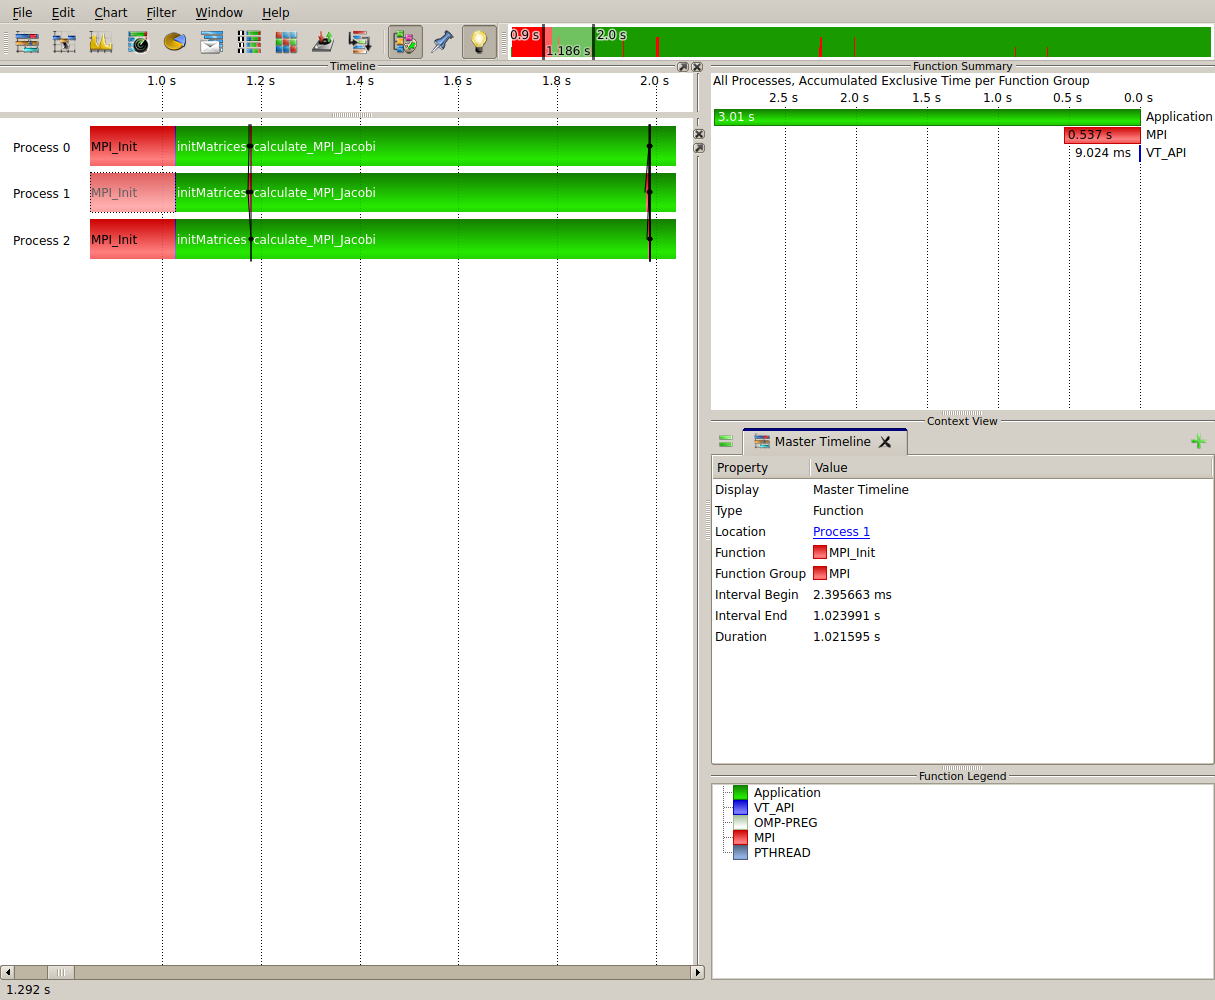
\includegraphics[scale=0.45]{./3_2_JA/Start.png}
 \caption{Der Beginn des Jacobi-Verfahrens bei 3 Prozessen}
\end{figure}
\begin{figure}[hr!]
 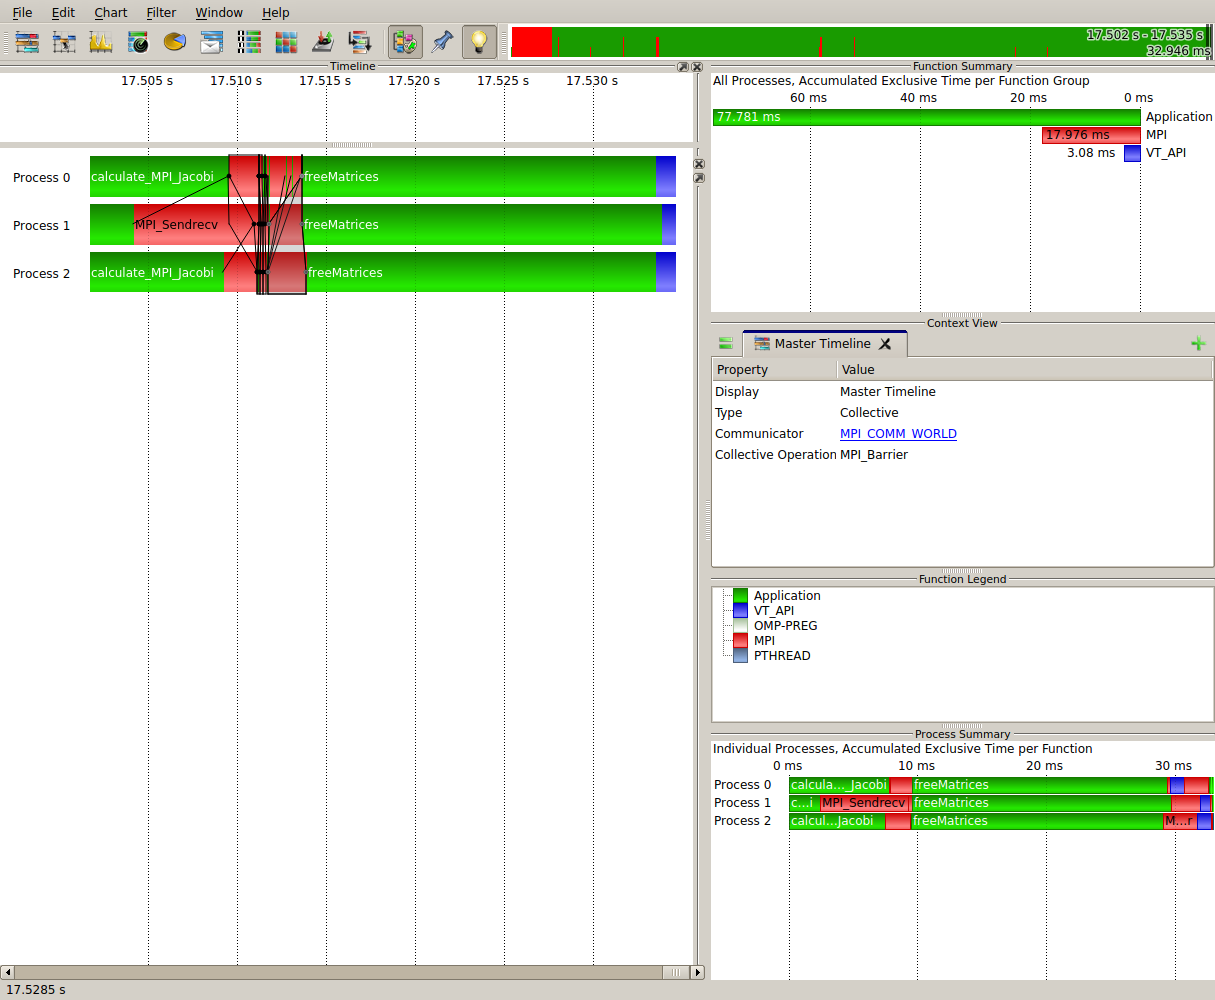
\includegraphics[scale=0.45]{./3_2_JA/End.png}
 \caption{Das Ende des Jacobi-Verfahrens bei 3 Prozessen}
\end{figure}

\begin{figure}[hr!]
 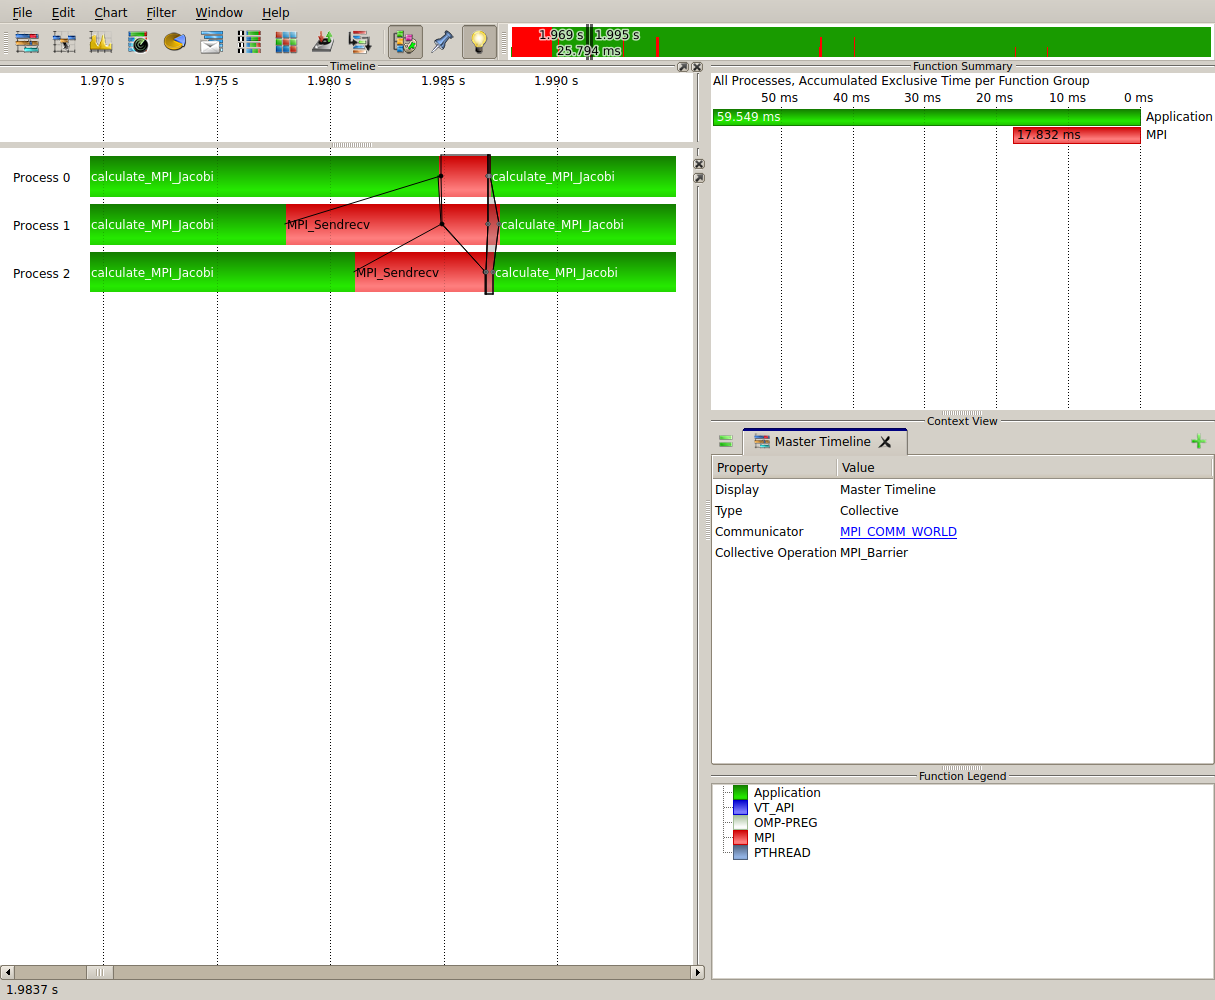
\includegraphics[scale=0.45]{./3_2_JA/Syncronize.png}
 \caption{Die Syncronisation am Ende eines Iterationsschrittes des Jacobi-Verfahrens bei 3 Prozessen}
\end{figure}

\subsubsection{4 Knoten 5 Prozesse}

\begin{figure}[hr!]
 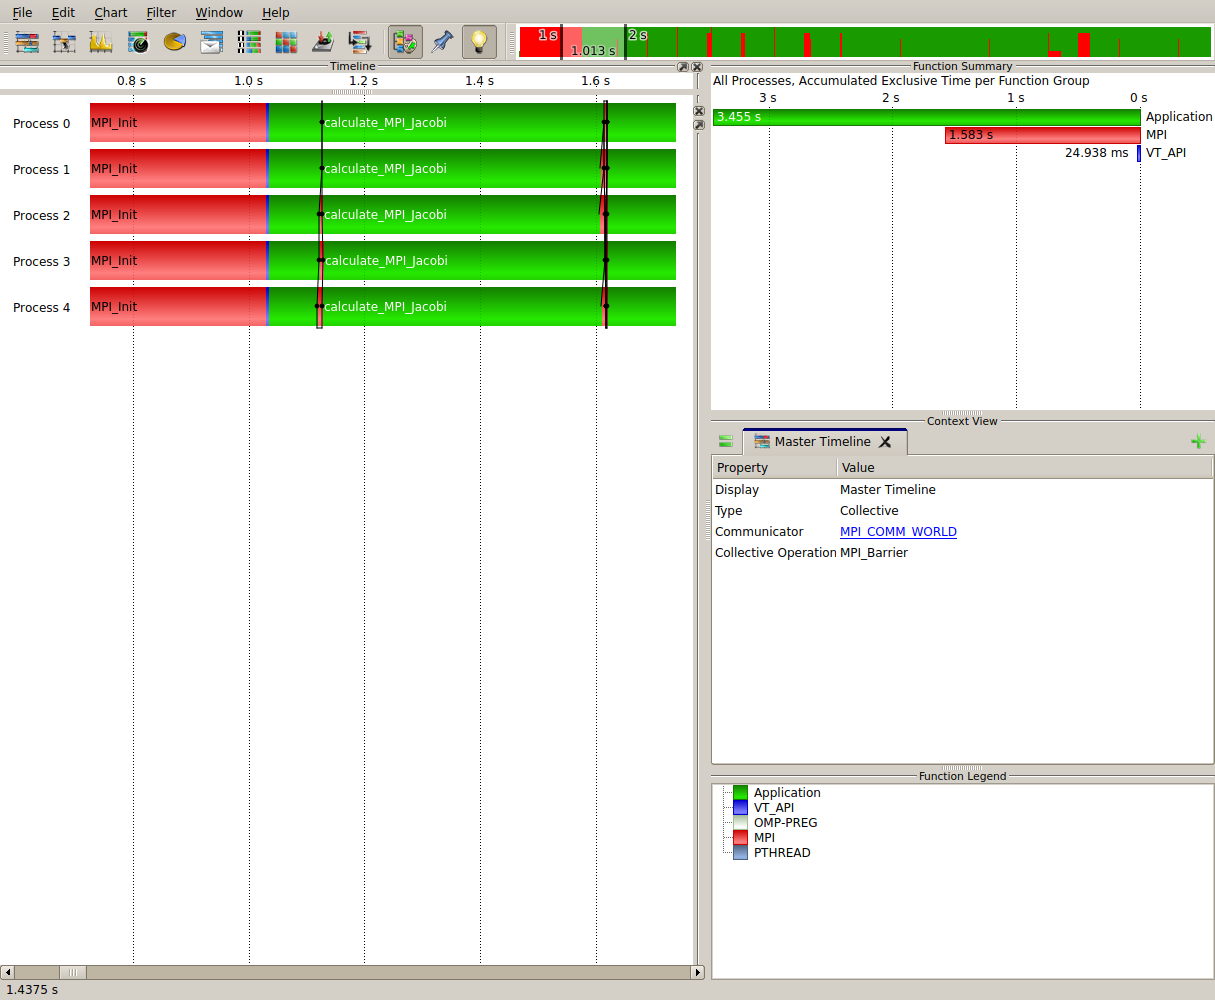
\includegraphics[scale=0.45]{./5_4_JA/Start.png}
 \caption{Der Beginn des Jacobi-Verfahrensbei 5 Prozessen}
\end{figure}
\begin{figure}[hr!]
 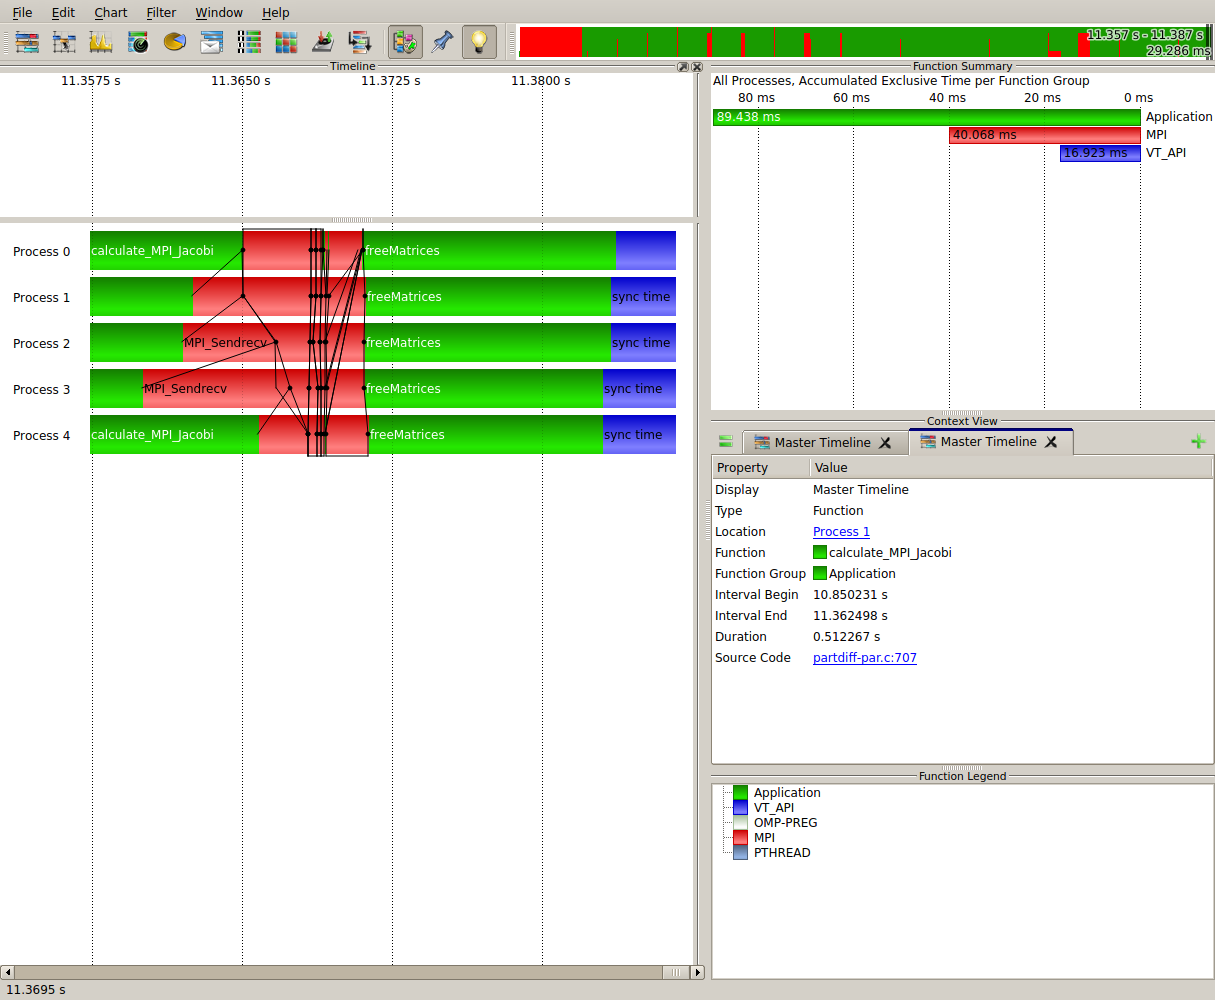
\includegraphics[scale=0.45]{./5_4_JA/End.png}
 \caption{Das Ende des Jacobi-Verfahrens bei 5 Prozessen}
\end{figure}

\begin{figure}[hr!]
 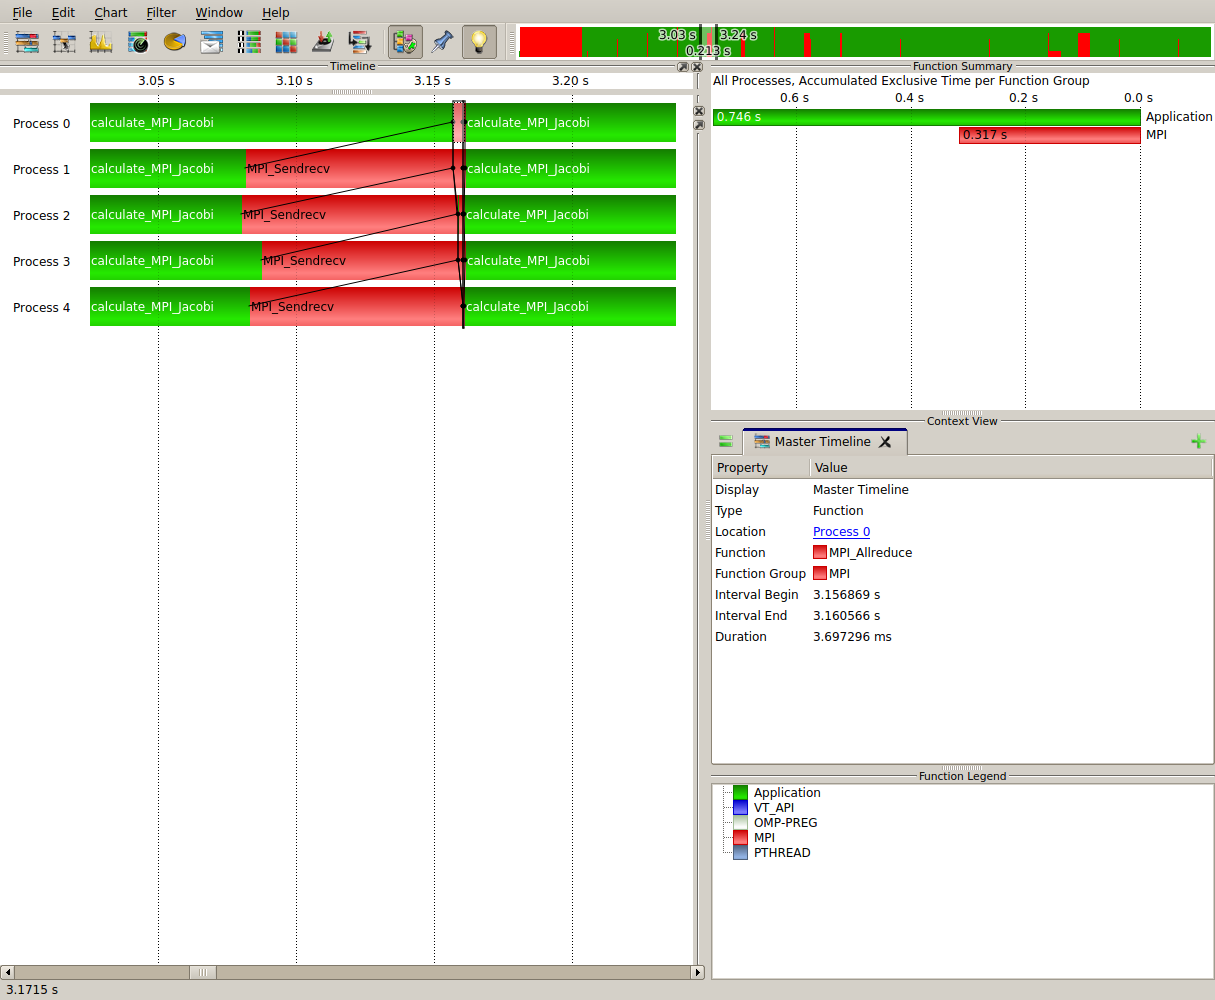
\includegraphics[scale=0.45]{./5_4_JA/Syncronize.png}
 \caption{Die Syncronisation am Ende eines Iterationsschrittes des Jacobi-Verfahrens bei 5 Prozessen}
\end{figure}

\newpage
\FloatBarrier
\subsection{Gauss-Seidel}
\subsubsection{2 Knoten 3 Prozesse}

\begin{figure}[hr!]
 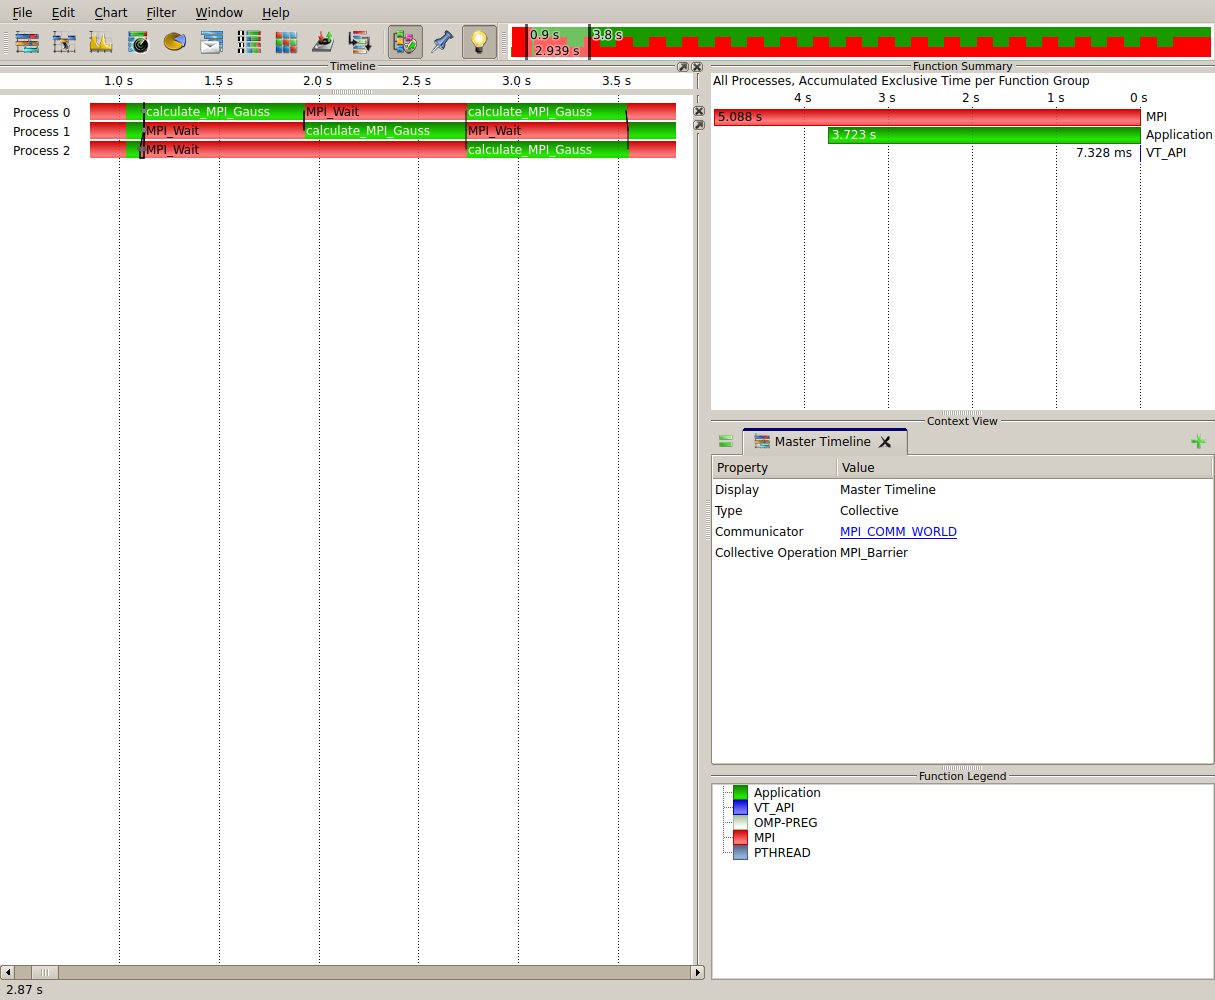
\includegraphics[scale=0.45]{./3_2_GS/Start.png}
 \caption{Der Beginn des Gauss-Seidel-Verfahren bei 3 Prozessen}
\end{figure}
\begin{figure}[hr!]
 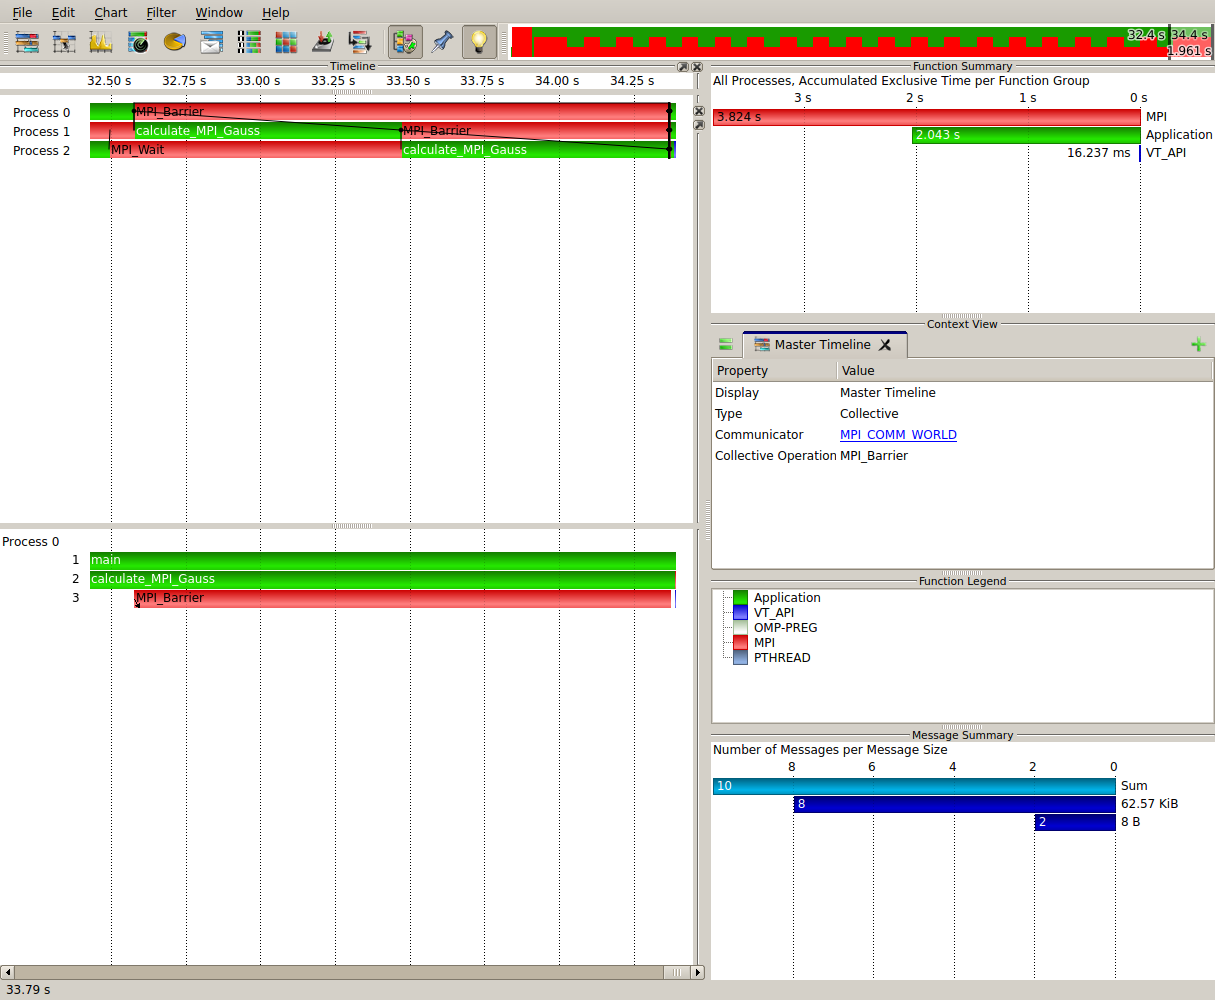
\includegraphics[scale=0.45]{./3_2_GS/End.png}
 \caption{Das Ende der Pipeline des Gauss-Seidel-Verfahren bei 3 Prozessen}
\end{figure}

\begin{figure}[hr!]
 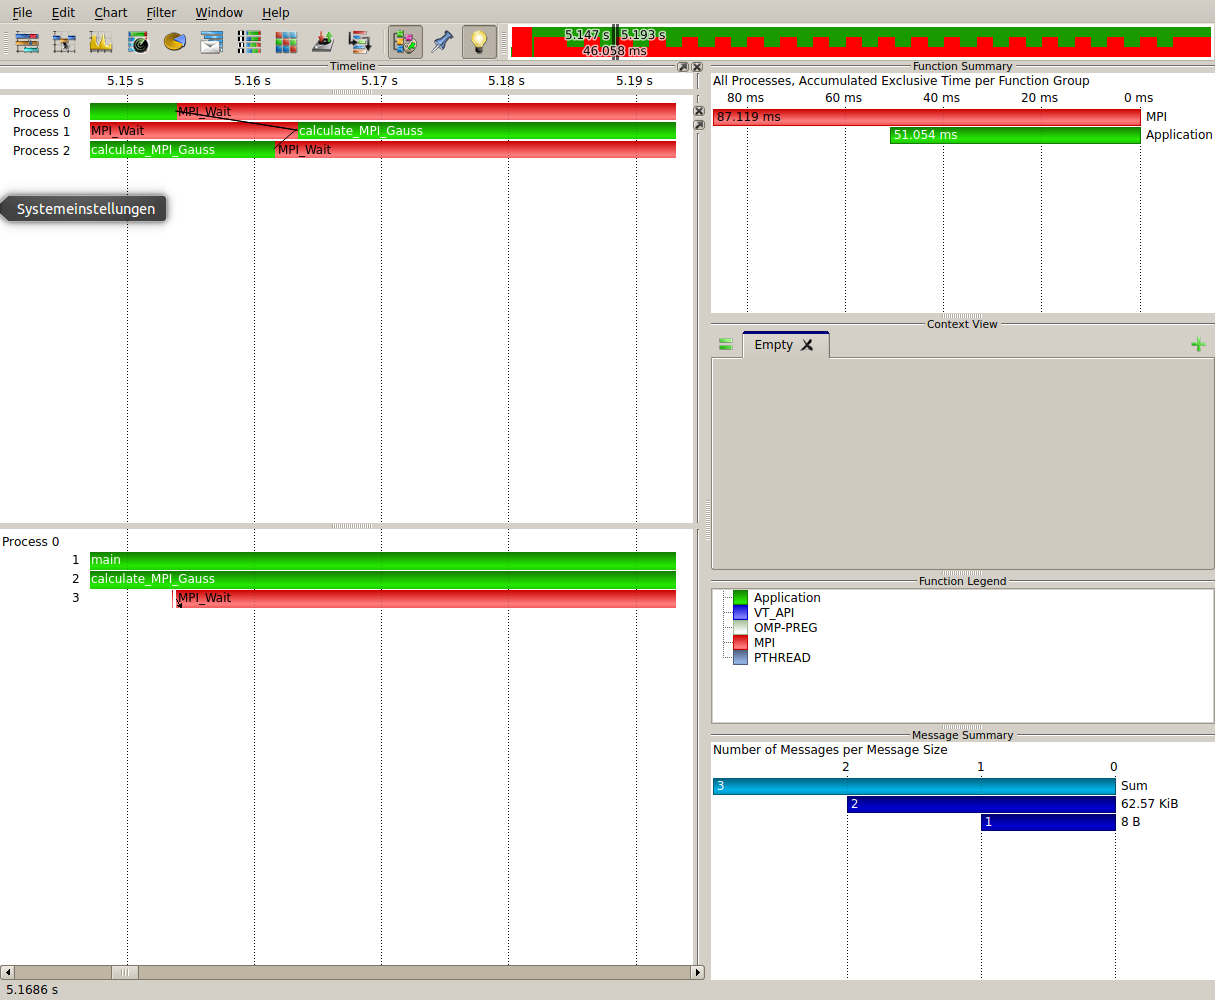
\includegraphics[scale=0.45]{./3_2_GS/Syncronize.png}
 \caption{Die Syncronisation am Ende eines Iterationsschrittes des Gauss-Seidel-Verfahren bei 3 Prozessen}
\end{figure}

\subsubsection{4 Knoten 5 Prozesse}

\begin{figure}[hr!]
 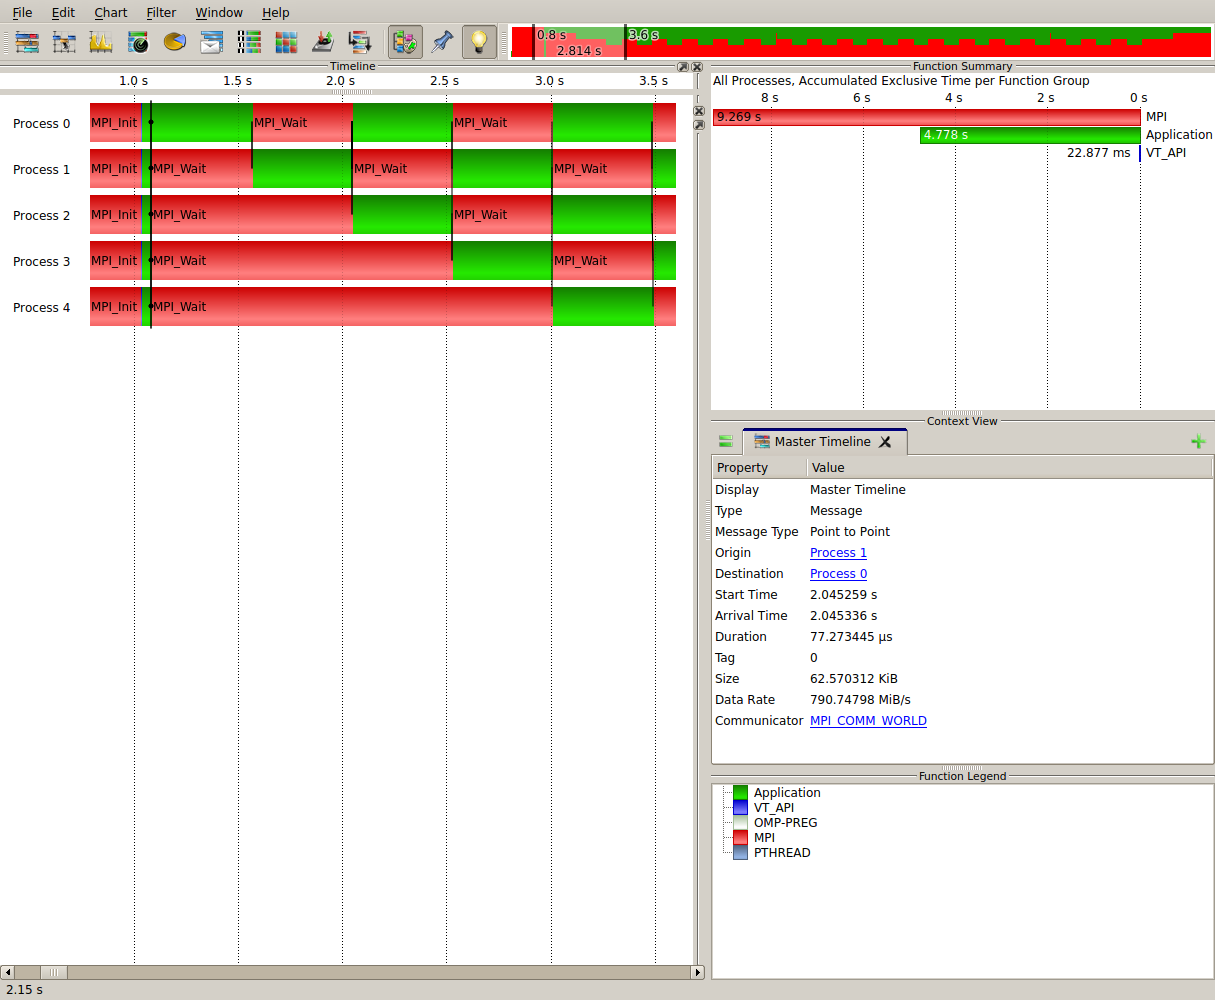
\includegraphics[scale=0.45]{./5_4_GS/Start.png}
 \caption{Der Beginn des Gauss-Seidel-Verfahren bei 5 Prozessen}
\end{figure}
\begin{figure}[hr!]
 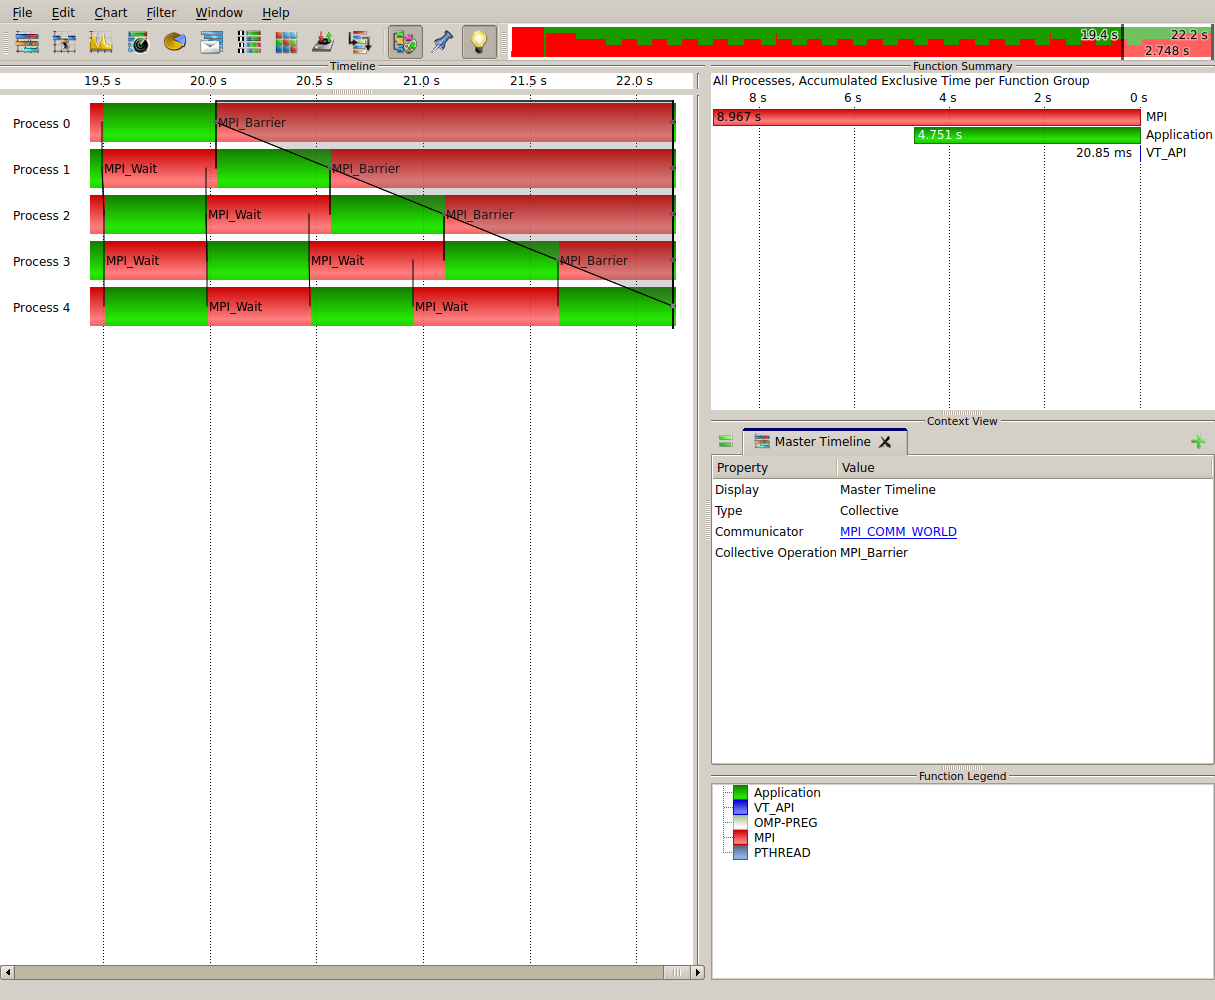
\includegraphics[scale=0.45]{./5_4_GS/End.png}
 \caption{Das Ende der Pipeline des Gauss-Seidel-Verfahren bei 5 Prozessen}
\end{figure}

\begin{figure}[hr!]
 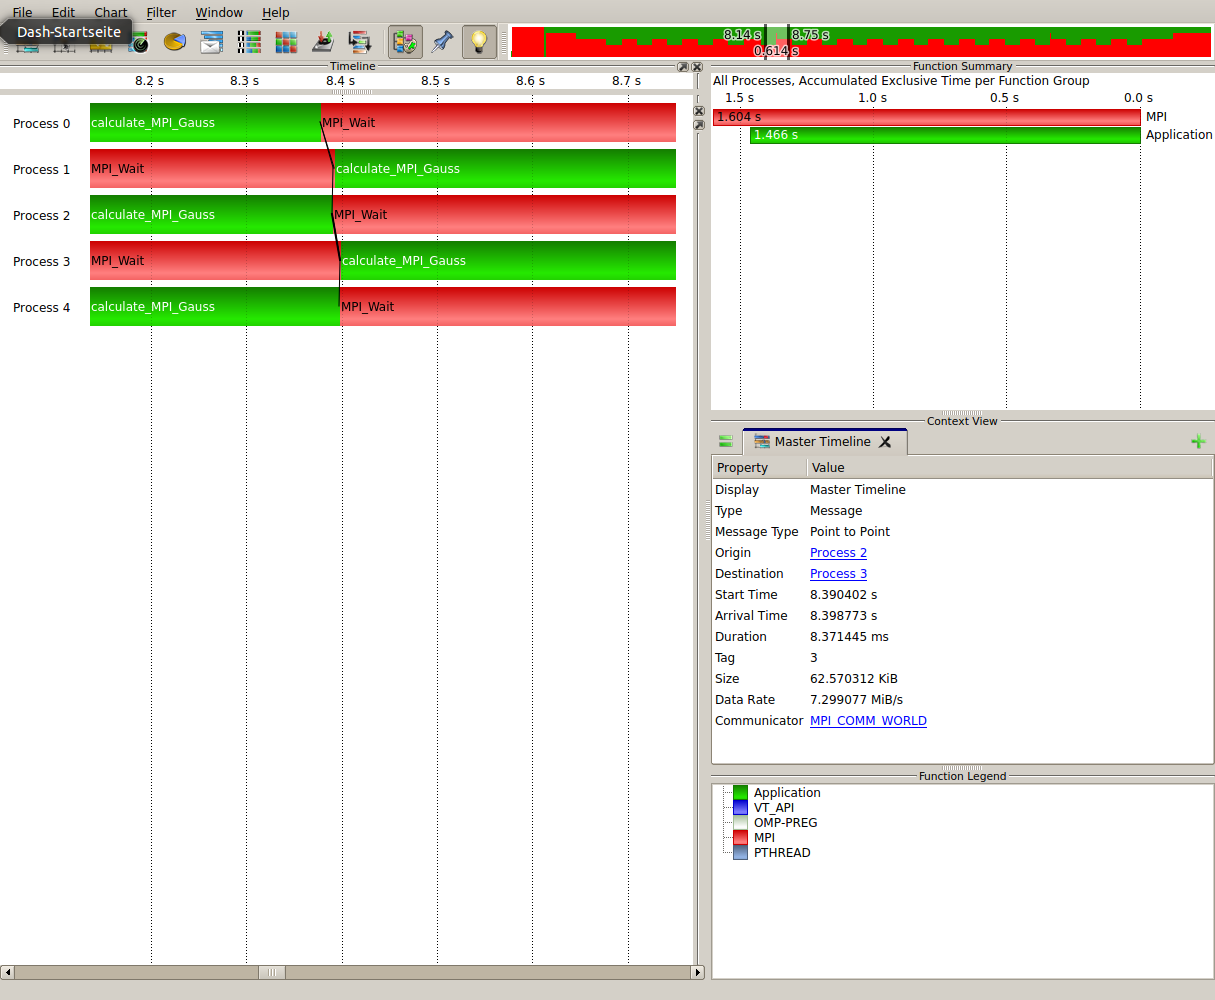
\includegraphics[scale=0.45]{./5_4_GS/Syncronize.png}
 \caption{Die Syncronisation am Ende eines Iterationsschrittes des Gauss-Seidel-Verfahren bei 5 Prozessen}
\end{figure}

\newpage
\FloatBarrier
\subsection{Diskussion}
Das Jacobi Verfahren hat in diesen Konfigurationen, die hier Visualisiert wurden kaum Probleme performant zu arbeiten Es kommt beim Jacobi-Verfahren nie vor, dass Desysncronisationen länger als einen Iterationsschritt andauern. Die ist eine Folge aus der Benutzung der Blockierenden Kommunikation von Allreduce und SendRecv, sodass alle Prozesse am Abschluss eines Iterationsschrittes aufeinander warten. 
Beim Gauss-Seidel-Verfahren ist durch das Pipelining anfälliger für Desyncronistation, leider ist sie auch wesentlich schwerer zu erkennen. Die Prozesse des Gauss-Seidel-Verfahrens scheinen sich ledoch größtenteils sehr gut dynamisch miteinander zu sysnchronisieren.
Ein Fehler in der Kommunikationsstruktur des Gauss-Seidel-Verfahrens wurde jedoch offenbar, da sich die Berechnnung jeweils mit einem Wait gleicher Länge abwechselt. Leider wird aus der Visualisierung nicht offenbar, in welcher Zeile des Programmcodes dieses spezifische Wait aufgerufen wird. Dies ergibt ein Schachbrettmuster. Dieses führt dazu, dass im Durchschnitt 50\% der Rechenzeit für Warten vergeudet wird. Eine Änderung des Verhaltens der spezifischen Wait funktion in ein Wait mittels Interrupt würde die Energieeffizienz der Berechnung mit dem Gauss-Seidel-Verfahren erhöhen, ohne dass Änderungen an der Kommunikationsstruktur und ggf. Algorithmus vorzunehmen sind.  
\end{document}